\clearpage
\twocolumn[{%
\rqparent
\subsection{Above chance against the training tokens of the language}
\label{app:rq00_chance_vs_train_tokens}

\noindent\begin{minipage}[t]{0.485\textwidth}
\vspace{0pt}
\paragraph{Research Question.} \emph{Does a benchmark task clear chance once the model has seen enough tokens of the task's language, and is it the exposure or the model size that decides?}

\paragraph{Setup.} We measure the share of cells above chance. A cell is one (task, size, language setting K), read at one of the ten evaluated tenths of the run. We use the seed-1904 runs of every data build and ladder, 90M--1.7B, at K $\in$ \{1, 2, 8, 15, 30, 50\}. The tasks are the benchmark tasks with a chance level in trained languages. BPB and the bBPB twins have no chance level and are left out. A cell is above chance when it passes the gate (the per-run Wilson test and the half-of-the-runs rule), applied at that tenth. A cell sits at the number of tokens of the task's language that the checkpoint had seen: the language's share of the build's mixture $\times$ the size's token budget $\times$ the tenth. We bin the cells three per decade of tokens. From these bins we read, per benchmark and answer format, the token count from which half or 90 \% of its cells are above chance (Table~\ref{tab:rq0_thresholds}). We then test whether leaving out the cells below that threshold changes how well an aggregate score ranks the designs (Table~\ref{tab:app_rq00_token_exclusion}).
\end{minipage}\hfill
\begin{minipage}[t]{0.485\textwidth}
\vspace{0pt}
\begin{rqfinding}
\textbf{1. Outside English, the share of cells above chance rises with every decade of the language's tokens from $10^{7}$ on.} But at matched tokens the larger model still clears chance more often. The share goes from 43 \% at $10^{7}$--$10^{8}$ tokens to 63 \% at $10^{10}$--$10^{11}$. At $10^{8}$--$10^{9}$ tokens it is 43 \% at 90M against 63 \% at 1.7B, so exposure is necessary but not sufficient. (Figure~\ref{fig:app_rq00_chance_vs_train_tokens}.)
\\
\\
\textbf{2. Pooled over every language, the curve peaks at $10^{8}$--$10^{9}$ tokens and falls after, because the top bins are mostly English.} It reads 52 \% at $10^{8}$--$10^{9}$, dips to 51 \% at $10^{9}$--$10^{10}$ and drops to 41 \% at $10^{10}$--$10^{11}$ (25,047 cells, 81 \% of them English).
\\
\\
\textbf{3. Without English, the share stays near 40 \% up to $10^{8}$ tokens and rises with every decade after.} Per decade: 40 \% ($10^{5}$, 77 cells), 41 \% ($10^{6}$), 43 \% ($10^{7}$), 53 \% ($10^{8}$), 62 \% ($10^{9}$), 63 \% ($10^{10}$, 4,820 cells).
\end{rqfinding}
\end{minipage}
\vspace{\baselineskip}
}]

\begin{figure*}[p]
\centering
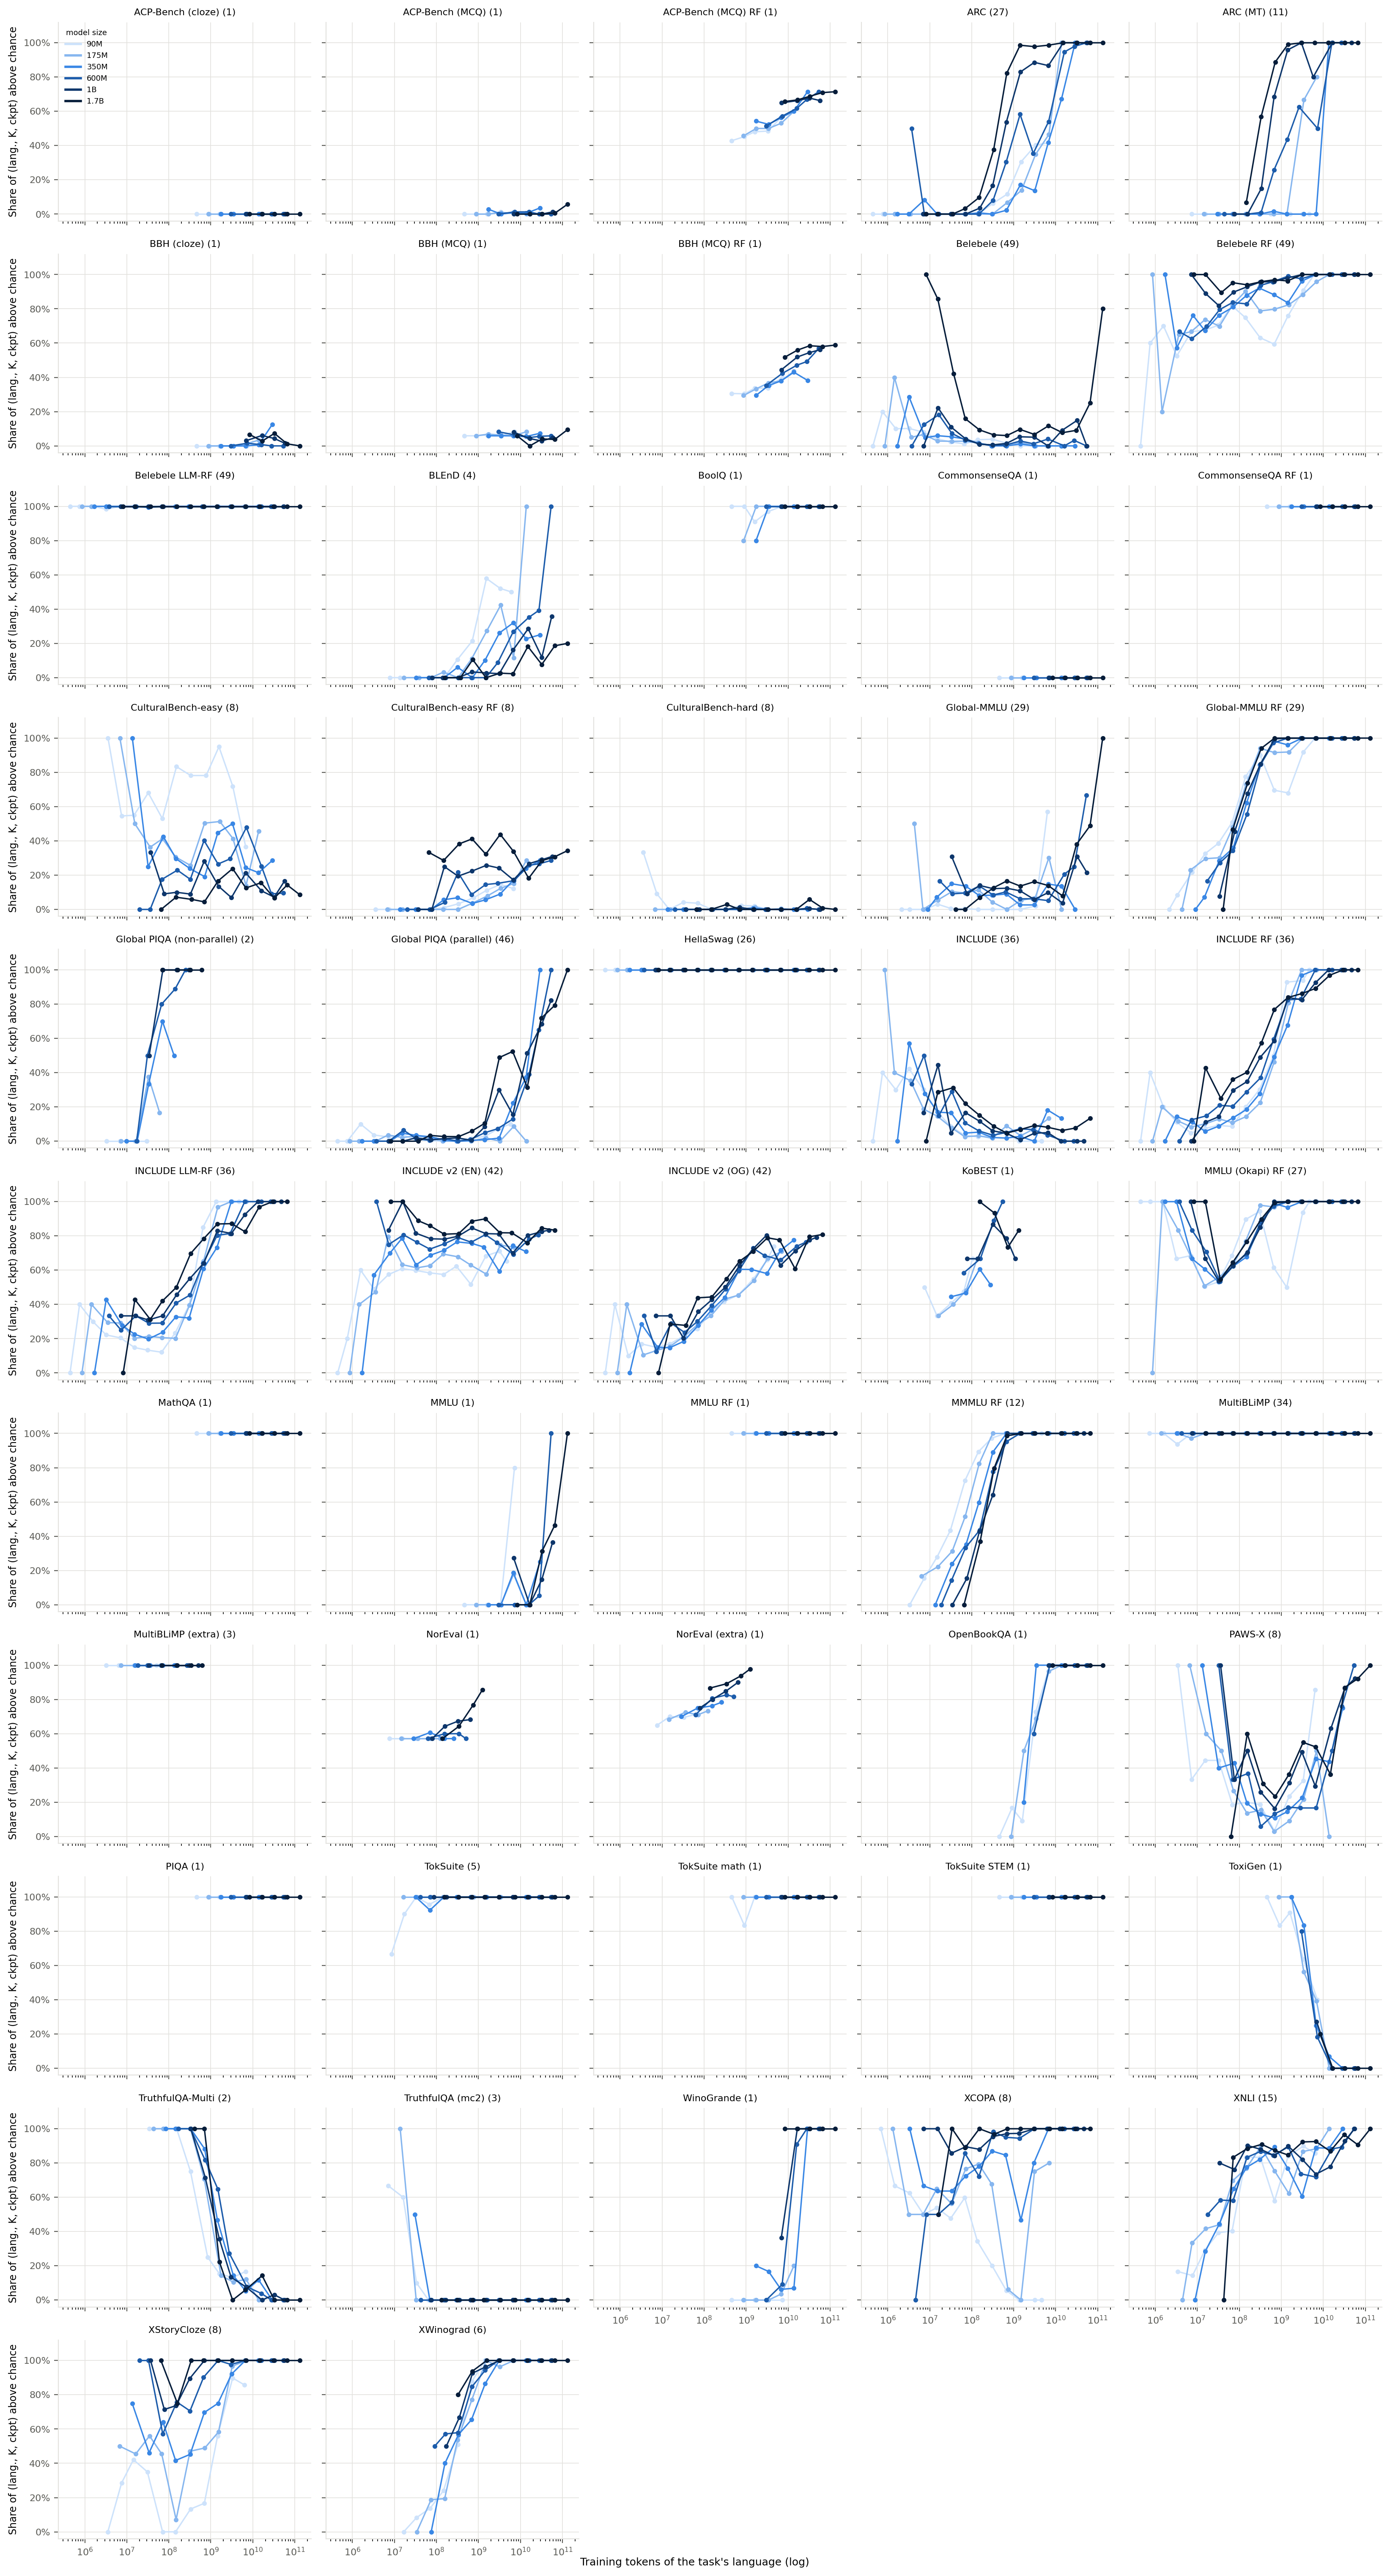
\includegraphics[width=\textwidth,height=0.8\textheight,keepaspectratio]{figures/app_rq00_chance_vs_train_tokens.png}
% source: src/signal-and-noise/analysis/rq00_chance_vs_train_tokens/pretraining/predictivity_seeds/pass_prob_vs_train_tokens_by_benchmark_1904_ckpts_paper.png
\caption{\textbf{Outside English, the share of cells above chance rises with every decade of the language's tokens from $10^{7}$ on.} One panel per benchmark (its number of tasks in parentheses). Each point is the share of (language, K, checkpoint) cells above chance, binned by the training tokens of the task's language that the checkpoint had seen (log scale). There is one line per model size, a darker blue for a larger size.}
\label{fig:app_rq00_chance_vs_train_tokens}
\end{figure*}

\begin{table*}[p]
\centering
\small
\begin{adjustbox}{max width=\textwidth}
\begin{tabular}{llrccccccrr}
\toprule
 & & & \multicolumn{2}{c}{All sizes} & \multicolumn{2}{c}{90M} & \multicolumn{2}{c}{1.7B} & & \\
\cmidrule(lr){4-5}\cmidrule(lr){6-7}\cmidrule(lr){8-9}
Benchmark & Format & Lang. & 50\% & 90\% & 50\% & 90\% & 50\% & 90\% & Margin & Items \\
\midrule
ARC & Original & 27 & $10^{9}$ & $2.2\times10^{10}$ & never & never & $4.6\times10^{8}$ & $10^{9}$ & 0.021 & 1{,}169 \\
\addlinespace
ARC (MT) & Original & 11 & $10^{9}$ & never & never & never & $\leq 2.2\times10^{8}$ & $10^{9}$ & 0.021 & 1{,}172 \\
\addlinespace
Belebele & Original & 49 & never & never & never & never & never & never & 0.024 & 900 \\
 & RF & 49 & $\leq 2.2\times10^{6}$ & $2.2\times10^{8}$ & $\leq 2.2\times10^{6}$ & $2.2\times10^{9}$ & $\leq 4.6\times10^{7}$ & $\leq 4.6\times10^{7}$ & 0.024 & 900 \\
 & LLM-RF & 49 & $\leq 2.2\times10^{6}$ & $\leq 2.2\times10^{6}$ & $\leq 2.2\times10^{6}$ & $\leq 2.2\times10^{6}$ & $\leq 4.6\times10^{7}$ & $\leq 4.6\times10^{7}$ & 0.024 & 898 \\
\addlinespace
BLEnD & Original & 4 & never & never & $2.2\times10^{9}$ & never & never & never & 0.032 & 500 \\
\addlinespace
CulturalBench-easy & Original & 8 & never & never & never & never & never & never & 0.157 & 25 \\
 & RF & 8 & never & never & never & never & never & never & 0.157 & 25 \\
\addlinespace
CulturalBench-hard & Original & 8 & never & never & never & never & never & never & 0.090 & 100 \\
\addlinespace
Global PIQA (non-parallel) & Original & 2 & $4.6\times10^{7}$ & $2.2\times10^{8}$ & -- & -- & -- & -- & 0.090 & 100 \\
\addlinespace
Global PIQA (parallel) & Original & 46 & $2.2\times10^{10}$ & never & never & never & $2.2\times10^{10}$ & never & 0.070 & 103 \\
\addlinespace
Global-MMLU & Original & 29 & never & never & never & never & never & never & 0.006 & 14{,}042 \\
 & RF & 29 & $10^{8}$ & $4.6\times10^{8}$ & $4.6\times10^{7}$ & $2.2\times10^{9}$ & $\leq 10^{8}$ & $2.2\times10^{8}$ & 0.006 & 14{,}042 \\
\addlinespace
HellaSwag & Original & 26 & $\leq 2.2\times10^{6}$ & $\leq 2.2\times10^{6}$ & $\leq 2.2\times10^{6}$ & $\leq 2.2\times10^{6}$ & $\leq 4.6\times10^{7}$ & $\leq 4.6\times10^{7}$ & 0.007 & 9{,}276 \\
\addlinespace
INCLUDE & Original & 36 & never & never & never & never & never & never & 0.032 & 548 \\
 & RF & 36 & $4.6\times10^{8}$ & $4.6\times10^{9}$ & $4.6\times10^{8}$ & never & $2.2\times10^{8}$ & $10^{10}$ & 0.032 & 548 \\
 & LLM-RF & 36 & $4.6\times10^{8}$ & $4.6\times10^{9}$ & $4.6\times10^{8}$ & never & $10^{8}$ & $10^{10}$ & 0.032 & 546 \\
\addlinespace
INCLUDE v2 (EN) & Original & 42 & $\leq 2.2\times10^{6}$ & never & $4.6\times10^{6}$ & never & $\leq 4.6\times10^{7}$ & never & 0.024 & 886 \\
\addlinespace
INCLUDE v2 (OG) & Original & 42 & $4.6\times10^{8}$ & never & $10^{9}$ & never & $2.2\times10^{8}$ & never & 0.024 & 886 \\
\addlinespace
MMLU (Okapi) & RF & 27 & $\leq 2.2\times10^{6}$ & $4.6\times10^{8}$ & $\leq 2.2\times10^{6}$ & never & $\leq 4.6\times10^{7}$ & $4.6\times10^{8}$ & 0.006 & 13{,}101 \\
\addlinespace
MMMLU & RF & 12 & $4.6\times10^{7}$ & $4.6\times10^{8}$ & $4.6\times10^{7}$ & $2.2\times10^{8}$ & $\leq 2.2\times10^{8}$ & $4.6\times10^{8}$ & 0.006 & 14{,}042 \\
\addlinespace
MultiBLiMP & Original & 34 & $\leq 2.2\times10^{6}$ & $\leq 2.2\times10^{6}$ & $\leq 2.2\times10^{6}$ & $\leq 2.2\times10^{6}$ & $\leq 4.6\times10^{7}$ & $\leq 4.6\times10^{7}$ & 0.017 & 2{,}291 \\
\addlinespace
MultiBLiMP (extra) & Original & 3 & $\leq 10^{7}$ & $\leq 10^{7}$ & -- & -- & -- & -- & 0.015 & 3{,}032 \\
\addlinespace
PAWS-X & Original & 8 & $2.2\times10^{10}$ & $4.6\times10^{10}$ & never & never & $2.2\times10^{10}$ & $4.6\times10^{10}$ & 0.018 & 2{,}000 \\
\addlinespace
TokSuite & Original & 5 & $\leq 2.2\times10^{7}$ & $\leq 2.2\times10^{7}$ & $\leq 2.2\times10^{7}$ & $\leq 2.2\times10^{7}$ & $\leq 4.6\times10^{8}$ & $\leq 4.6\times10^{8}$ & 0.125 & 40 \\
\addlinespace
TruthfulQA (mc2) & Original & 3 & never & never & never & never & never & never & 0.030 & 788 \\
\addlinespace
TruthfulQA-Multi & Original & 2 & never & never & never & never & never & never & 0.024 & 817 \\
\addlinespace
XCOPA & Original & 8 & $\leq 4.6\times10^{6}$ & $4.6\times10^{9}$ & never & never & $\leq 10^{8}$ & $\leq 10^{8}$ & 0.038 & 500 \\
\addlinespace
XNLI & Original & 15 & $4.6\times10^{7}$ & $2.2\times10^{10}$ & $10^{8}$ & never & $\leq 10^{8}$ & $2.2\times10^{10}$ & 0.016 & 2{,}490 \\
\addlinespace
XStoryCloze & Original & 8 & $2.2\times10^{8}$ & $2.2\times10^{9}$ & $10^{9}$ & never & $\leq 2.2\times10^{8}$ & $\leq 2.2\times10^{8}$ & 0.022 & 1{,}511 \\
\addlinespace
XWinograd & Original & 6 & $2.2\times10^{8}$ & $10^{9}$ & $2.2\times10^{8}$ & $10^{9}$ & $\leq 10^{9}$ & $\leq 10^{9}$ & 0.043 & 410 \\
\bottomrule
\end{tabular}

\end{adjustbox}
% source: src/signal-and-noise/analysis/rq00_chance_vs_train_tokens/pretraining/predictivity_seeds/pass_threshold_tokens_by_benchmark_1904_ckpts.tex
\caption{\textbf{Training tokens of the language from which a benchmark is above chance.} For each multilingual benchmark (trained in at least two languages) and answer format, the lower edge of the token bin from which the share of (language, $K$, checkpoint) cells above chance is at least 50\% or 90\% in that bin and in every larger bin, pooled over the model sizes 90M--1.7B and for the 90M and 1.7B models alone. Bins are three per decade of the training tokens of the language that the checkpoint had seen, and a bin counts only with at least 20 cells. $\leq$ marks a level already met in the first bin, never a level that is not reached. Lang. is the number of trained languages. Margin is the median accuracy above chance that a task needs for its Wilson bound to clear chance, and Items its median item count. Seed-1904 runs of every data build and ladder, every evaluated tenth of a run. The pooled bins mix sizes, and from $10^{10}$ tokens on, most of their cells are English.}
\label{tab:rq0_thresholds}
\end{table*}

\begin{table*}[p]
\centering
\small
\begin{adjustbox}{max width=\textwidth}
\begin{tabular}{lccccc}
\toprule
 & \multicolumn{2}{c}{SE of the aggregate} & \multicolumn{3}{c}{DA-size, single-axis pairs} \\
\cmidrule(lr){2-3}\cmidrule(lr){4-6}
Size & All cells & Above threshold & All cells & Above threshold & Above chance \\
\midrule
90M & 0.008 & 0.010 & 0.748 & 0.677 & 0.692 \\
175M & 0.009 & 0.011 & 0.739 & 0.701 & 0.700 \\
350M & 0.010 & 0.011 & 0.761 & 0.736 & 0.730 \\
600M & 0.012 & 0.013 & 0.783 & 0.747 & 0.750 \\
1B & 0.014 & 0.014 & 0.810 & 0.762 & 0.774 \\
1.7B & 0.015 & 0.016 & -- & -- & -- \\
\bottomrule
\end{tabular}

\end{adjustbox}
% source: src/signal-and-noise/analysis/rq00_chance_vs_train_tokens/pretraining/predictivity/token_exclusion_da_size_mono_axis.tex
\caption{\textbf{Leaving out the cells below the token threshold lowers the decision accuracy of an aggregate score.} For each benchmark and each seed-1904 run at its final checkpoint, the aggregate is the mean of the benchmark's tasks over the languages the run trains. We compute it on every cell, on the cells at or above the benchmark's pooled 50\% token threshold (Table~\ref{tab:rq0_thresholds}), and on the cells above chance at the run's size and at 1.7B. SE is the median over runs of the standard deviation of the per-language values divided by the square root of their number. DA-size compares the aggregate of each proxy with the 1.7B aggregate under the same rule, on single-axis pairs, pooled over the 18 benchmarks that keep an aggregate under every rule. The nine benchmarks that never reach their threshold lose every cell.}
\label{tab:app_rq00_token_exclusion}
\end{table*}
